\documentclass[fleqn]{article}
\usepackage{amsmath}
\usepackage[dvips]{graphicx}
\bibliographystyle{plain}
%__________________________________
\begin{document}

\section*{\center Mach 2 Wedge}
\subsection*{\underline{Problem Description}}
This is a simulation of a symmetric $20^o$ wedge traveling through initially
quiescent air at Mach 2.0.  A shock forms at the leading edge of the
wedge and an expansion fan over its top.  Consultation of oblique shock
tables, e.g.~\cite{Saad} (pp.308-309) reveals that the angle of the leading
shock compares quite well with the expected value.  In addition, this
simulation demonstrates a few other useful features of the fluid-structure
interaction capability.  In this case, the structure is rigid, and as
such, essentially provides a boundary condition to the compressible flow
calculation.  Furthermore, the geometry of the wedge is described via a
triangulated surface, rather than the geometric primitives usually used.
This allows the user to study flow around arbitrarily complex objects,
without the difficulty of generating a body fitted mesh around that object.

\subsection*{\underline{Simulation Specifics}}
\begin{description} 
\item [Component used:] \hfill rmpmice (Rigid MPM-ICE)
\item [Input file name:] \hfill Mach2Wedge.ups
\item [Command used to run input file:]\hfill sus Mach2Wedge.ups
(Note: The files wedge40.pts and wedge40.tri must also be copied to
the same directory as sus.)

\item [Simulation Domain:]\hfill    0.25 x 0.0375 x 0.001 m

\item [Cell Spacing:]\hfill \\ 
.0005 x .0005 x .001 m (Level 0)

\item [Example Runtimes:] \hfill \\
 ~1.5 hours   (1 processor, 3.0 GHz Xeon)\\

\item [Physical time simulated:] \hfill 0.64 milliseconds

\item [Associate scirun network:] \hfill Mach2wedge.srn

\end{description}

\section*{\underline{Results}}

Figure~\ref{figwedge} shows a snapshot of the simulation.  Contour
plot depicts pressure and reflects the presence of a leading shock
and an expansion fan.
\begin{figure}[b]
  \center
%  \scalebox{0.2}{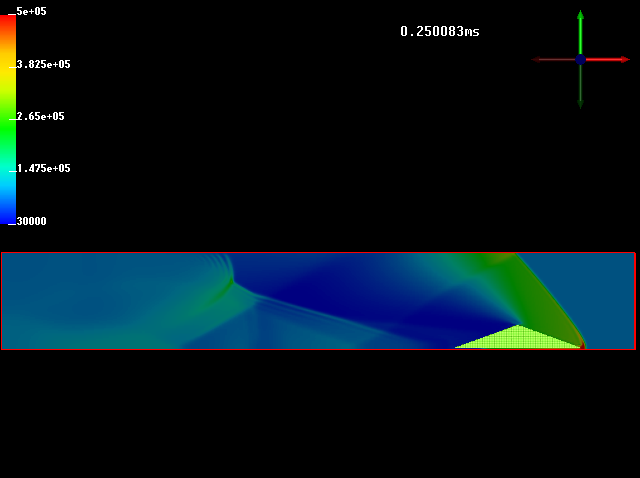
\includegraphics{Mach2Wedge.png}}
  \caption{$20^o$ wedge moving at Mach 2.0 through initially stationary
air.  Contour plot depicts pressure.}
  \label{figdisks}
\end{figure}

\bibliography{../references}

\end{document}
